\chapter{Metodología}
% ==============================================================================
% 4.1 BLOQUES SEMÁNTICOS
% ==============================================================================
\section{Definición y estructuración de bloques semánticos}
\label{sec:bloques_semanticos}

El capítulo anterior evidenció tres limitaciones estructurales del enfoque determinístico y sintáctico:

\begin{itemize}
    \item La dependencia del expediente como primer filtro en ausencia de identificadores únicos confiables.
    \item El riesgo de falsos positivos y falsos negativos inducido por la ambigüedad de la captura manual en los nombres y apellidos, que no resuelve la normalización.
    \item La heterogeneidad estructural que impide comparar directamente los registros completos columna a columna entre bases de datos distintas.
\end{itemize}

La más crítica para el diseño de un sistema de ligado automático es la tercera: una misma variable real (el diagnóstico del paciente, su ocupación, su nivel socioeconómico) se representa en cada sistema del INER con esquemas, vocabularios y formatos distintos. Comparar caracteres entre campos que no comparten ni nombre, ni tipo, ni codificación es un callejón sin salida metodológico. La alternativa metodológica que se propone en este capítulo consiste en trascender la representación tabular y operar sobre una \textbf{abstracción semántica} del paciente, donde la información del registro quede representada de manera uniforme y comparable entre bases de datos.

Para ello, se define el concepto de \textbf{bloque semántico} como una agrupación lógica de atributos que comparten un eje de información común, independientemente de la nomenclatura u organización de la base de datos de origen. Cada bloque se materializa en una fuente particular mediante un \textit{soporte}, que es el subconjunto de columnas que lo implementan en esa base específica.

La noción de bloque semántico puede entenderse por analogía con las modalidades de un modelo multimodal. Por ejemplo, en un sistema de clasificación musical, la calidad de la predicción mejora cuando el modelo dispone simultáneamente de la señal de audio, la letra de la canción y el video oficial. Cada una de estas fuentes ofrece una vista parcial de la misma realidad subyacente, y su combinación enriquece la representación que el modelo puede aprender. Sin embargo, no toda canción tiene video oficial; algunas tienen letra, otras no. Un modelo multimodal robusto debe operar con las modalidades disponibles en cada caso, sin depender de que todas estén siempre presentes.

Los bloques semánticos cumplen el mismo rol en el dominio de resolución de entidades en el ámbito clínico. \texttt{[BLK\_ID]} es una modalidad que identifica al paciente, \texttt{[BLK\_CLIN]} es otra que caracteriza su perfil clínico, \texttt{[BLK\_GEO]} otra con información extra, y así sucesivamente. Cada base de datos del INER implementa un subconjunto distinto de estas modalidades: Comorbilidad carece de \texttt{[BLK\_GEO]} y \texttt{[BLK\_SOCIO]} por diseño, del mismo modo que una canción puede carecer de video oficial. Cuando el paciente es atendido en múltiples servicios, sus modalidades se distribuyen entre los sistemas, y es tarea del modelo de ligado reconstruir la unidad de la entidad a partir de las piezas disponibles. La serialización basada en bloques, que se detalla en la Sección~\ref{sec:early_fusion}, materializa esta filosofía: cada registro se representa únicamente con los bloques que posee, produciendo secuencias de longitud variable que reflejan fielmente la información presente sin imputación ni relleno.

% Diagrama: Bloques semánticos como modalidades del paciente
\begin{figure}[H]
\centering
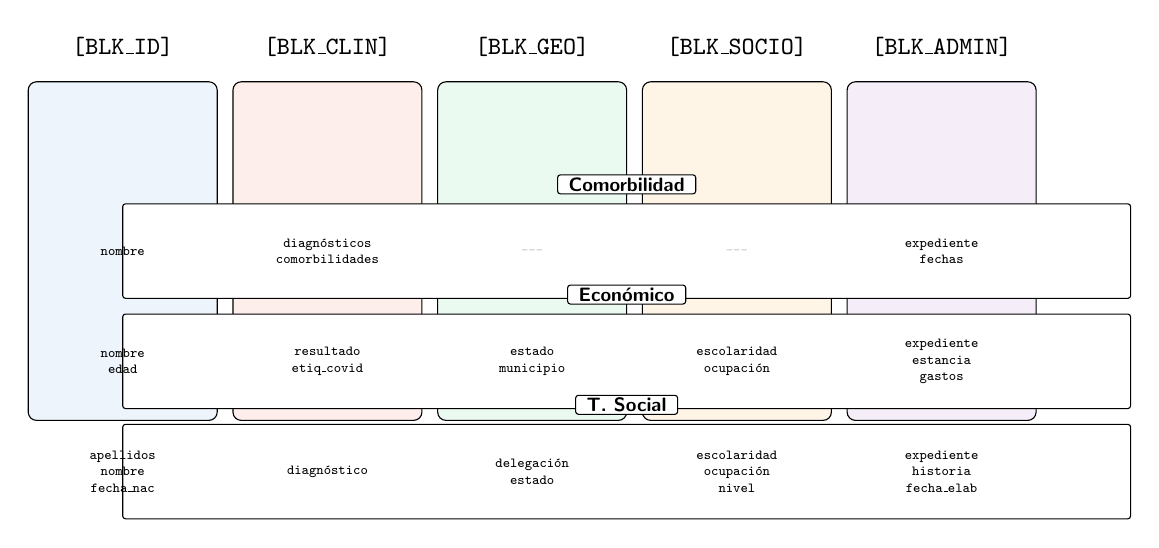
\begin{tikzpicture}[
    cell/.style={align=center, font=\tiny\ttfamily},
    rowbox/.style={draw, rounded corners=1pt, fill=white, inner sep=5pt},
    bloc/.style={draw, rounded corners=3pt, inner sep=2pt},
    rowlabel/.style={anchor=east, font=\footnotesize\sffamily},
    tab/.style={draw, rounded corners=1pt, fill=white, inner xsep=4pt, inner ysep=1pt, font=\scriptsize\sffamily\bfseries}]

\definecolor{cID}{HTML}{4A90D9}
\definecolor{cCLIN}{HTML}{E74C3C}
\definecolor{cGEO}{HTML}{2ECC71}
\definecolor{cSOCIO}{HTML}{F39C12}
\definecolor{cADMIN}{HTML}{9B59B6}

\pgfmathsetmacro{\cw}{2.4}
\pgfmathsetmacro{\cs}{0.2}
\pgfmathsetmacro{\rh}{1.2}
\pgfmathsetmacro{\rs}{0.2}

\pgfmathsetmacro{\xA}{0}
\pgfmathsetmacro{\xB}{\cw+\cs}
\pgfmathsetmacro{\xC}{2*(\cw+\cs)}
\pgfmathsetmacro{\xD}{3*(\cw+\cs)}
\pgfmathsetmacro{\xE}{4*(\cw+\cs)}
\pgfmathsetmacro{\tw}{5*\cw+4*\cs}
\pgfmathsetmacro{\bw}{\cw}
\pgfmathsetmacro{\bh}{3*\rh+2*\rs+0.3}

\pgfmathsetmacro{\yA}{0}
\pgfmathsetmacro{\yB}{-\rh-\rs}
\pgfmathsetmacro{\yC}{-2*\rh-2*\rs}

% BARRAS VERTICALES (bloques)
\node[bloc, fill=cID!10,   minimum width=\bw*1cm, minimum height=\bh*1cm] at (\xA*1cm, 0) {};
\node[bloc, fill=cCLIN!10, minimum width=\bw*1cm, minimum height=\bh*1cm] at (\xB*1cm, 0) {};
\node[bloc, fill=cGEO!10,  minimum width=\bw*1cm, minimum height=\bh*1cm] at (\xC*1cm, 0) {};
\node[bloc, fill=cSOCIO!10,minimum width=\bw*1cm, minimum height=\bh*1cm] at (\xD*1cm, 0) {};
\node[bloc, fill=cADMIN!10,minimum width=\bw*1cm, minimum height=\bh*1cm] at (\xE*1cm, 0) {};

% Etiquetas de bloques (arriba)
\node[above=2mm, font=\small\ttfamily\bfseries] at (\xA*1cm, 0.5*\bh*1cm) {\texttt{[BLK\_ID]}};
\node[above=2mm, font=\small\ttfamily\bfseries] at (\xB*1cm, 0.5*\bh*1cm) {\texttt{[BLK\_CLIN]}};
\node[above=2mm, font=\small\ttfamily\bfseries] at (\xC*1cm, 0.5*\bh*1cm) {\texttt{[BLK\_GEO]}};
\node[above=2mm, font=\small\ttfamily\bfseries] at (\xD*1cm, 0.5*\bh*1cm) {\texttt{[BLK\_SOCIO]}};
\node[above=2mm, font=\small\ttfamily\bfseries] at (\xE*1cm, 0.5*\bh*1cm) {\texttt{[BLK\_ADMIN]}};

% Renglón 1: Comorbilidad
\node[rowbox, minimum width=\tw*1cm, minimum height=\rh*1cm] at (0.5*\tw*1cm, \yA*1cm) {};
\node[tab, anchor=south] at (0.5*\tw*1cm, \yA*1cm + 0.5*\rh*1cm + 0.12cm) {Comorbilidad};
\node[cell] at (\xA*1cm, \yA*1cm) {nombre};
\node[cell] at (\xB*1cm, \yA*1cm) {diagnósticos\\comorbilidades};
\node[cell, text=gray!40] at (\xC*1cm, \yA*1cm) {---};
\node[cell, text=gray!40] at (\xD*1cm, \yA*1cm) {---};
\node[cell] at (\xE*1cm, \yA*1cm) {expediente\\fechas};

% Renglón 2: Económico
\node[rowbox, minimum width=\tw*1cm, minimum height=\rh*1cm] at (0.5*\tw*1cm, \yB*1cm) {};
\node[tab, anchor=south] at (0.5*\tw*1cm, \yB*1cm + 0.5*\rh*1cm + 0.12cm) {Económico};
\node[cell] at (\xA*1cm, \yB*1cm) {nombre\\edad};
\node[cell] at (\xB*1cm, \yB*1cm) {resultado\\etiq\_covid};
\node[cell] at (\xC*1cm, \yB*1cm) {estado\\municipio};
\node[cell] at (\xD*1cm, \yB*1cm) {escolaridad\\ocupación};
\node[cell] at (\xE*1cm, \yB*1cm) {expediente\\estancia\\gastos};

% Renglón 3: Trabajo Social
\node[rowbox, minimum width=\tw*1cm, minimum height=\rh*1cm] at (0.5*\tw*1cm, \yC*1cm) {};
\node[tab, anchor=south] at (0.5*\tw*1cm, \yC*1cm + 0.5*\rh*1cm + 0.12cm) {T. Social};
\node[cell] at (\xA*1cm, \yC*1cm) {apellidos\\nombre\\fecha\_nac};
\node[cell] at (\xB*1cm, \yC*1cm) {diagnóstico};
\node[cell] at (\xC*1cm, \yC*1cm) {delegación\\estado};
\node[cell] at (\xD*1cm, \yC*1cm) {escolaridad\\ocupación\\nivel};
\node[cell] at (\xE*1cm, \yC*1cm) {expediente\\historia\\fecha\_elab};

\end{tikzpicture}
\caption{Bloques semánticos como modalidades. Las columnas verticales representan los cinco bloques;
las franjas horizontales son registros de cada base. Las intersecciones muestran ejemplos del soporte;
las celdas vacías (\texttt{---}) indican bloques ausentes por diseño.}
\label{fig:bloques_modalidades}
\end{figure}


El análisis de los tres sistemas del INER, documentado en el Anexo de Bloques Semánticos, identificó cinco bloques que cubren la totalidad de la información de los pacientes. La Tabla~\ref{tab:columnas_por_bloque_comparativo} muestra el mapeo completo de columnas a bloques para cada fuente.

\begin{table}[H]
\centering
\caption{Columnas por bloque semántico — comparativa entre fuentes}
\label{tab:columnas_por_bloque_comparativo}
\small
\resizebox{\linewidth}{!}{%
\begin{tabular}{>{\raggedright\arraybackslash}p{3cm}
                >{\raggedright\arraybackslash}p{5.5cm}
                >{\raggedright\arraybackslash}p{5.5cm}
                >{\raggedright\arraybackslash}p{5.5cm}}
\toprule
\textbf{Bloque semántico} & \textbf{Comorbilidad} & \textbf{Económico} & \textbf{Trabajo Social} \\
\midrule
\texttt{[BLK\_ID]}
  & \texttt{nombre}
  & \texttt{NOMBRE\_DEL\_PACIENTE}, \texttt{SEXO}, \texttt{EDAD}, \texttt{GRUPO\_EDAD}
  & \texttt{APELLIDO PATERNO}, \texttt{APELLIDO MATERNO}, \texttt{NOMBRE}, \texttt{EDAD}, \texttt{FECHA DE NACIMIENTO}, \texttt{GENERO} \\
\midrule
\texttt{[BLK\_CLIN]}
  & \texttt{diagnosticoprincipal}, \texttt{diagnostico2}, \texttt{diagnostico3}, \texttt{diagnostico4}, \texttt{cie10}, \texttt{cie102}, \texttt{cie103}, \texttt{cie104}, \texttt{dx2}, \texttt{dx3}, \texttt{dx4}, \texttt{comorbi}, \texttt{comorbicv}, \texttt{obesidad}, \texttt{obesidad1}, \texttt{cardiopatia}, \texttt{diabetes}, \texttt{nefropatia}, \texttt{eaperge}, \texttt{tephap}
  & \texttt{RESULTADO}, \texttt{ETIQUETAS\_COVID}, \texttt{MOTIVO\_DE\_EGRESO}
  & \texttt{DIAGNOSTICO} \\
\midrule
\texttt{[BLK\_GEO]}
  & ---
  & \texttt{ESTADO\_RESIDENCIA}, \texttt{MUNICIPIO\_RESIDENCIA}, \texttt{CLAVE GEOESTADISTICA} (estatal y municipal)
  & \texttt{DELEGACIÓN O MUNICIPIO PERMANENTE}, \texttt{ESTADO / PAIS PERMANENTE} \\
\midrule
\texttt{[BLK\_SOCIO]}
  & ---
  & \texttt{ESCOLARIDAD}, \texttt{OCUPACION}, \texttt{DERECHOHABIENTE Y/O BENEFICIARIO}, \texttt{NIVEL\_SOCIOECONOMICO}, \texttt{VULNERABILIDAD\_SOCIOECONOMICA}
  & \texttt{ESCOLARIDAD}, \texttt{OCUPACIÓN}, \texttt{DERECHOHABIENTE Y/O BENEFICIARIO}, \texttt{TOTAL DE PUNTOS}, \texttt{NIVEL SOCIOECONÓMICO} \\
\midrule
\texttt{[BLK\_ADMIN]}
  & \texttt{expediente}, \texttt{fechaing}, \texttt{fechaegr}
  & \texttt{EXP}, \texttt{DIAS\_ESTANCIA}, \texttt{FECHA\_INGRESO\_INER}, \texttt{FECHA\_DE\_ALTA\_MEJORIA}, \texttt{TOTAL\_DE\_INGRESOS}, \texttt{TOTAL\_DE\_EGRESOS}, \texttt{GASTO\_TOTAL}, \texttt{GASTO\_DIARIO}
  & \texttt{EXPEDIENTE}, \texttt{NO. HISTORIA}, \texttt{FECHA DE ELABORACIÓN}, \texttt{AÑO}, \texttt{FILA} \\
\bottomrule
\end{tabular}}
\end{table}

La tabla revela dos formas de heterogeneidad. La primera es cuantitativa: un mismo bloque tiene distinto número de columnas según la fuente. \texttt{[BLK\_ID]} va de 1 columna en Comorbilidad a 6 en Trabajo Social; \texttt{[BLK\_CLIN]} va de 20 columnas en Comorbilidad a 1 en Trabajo Social. La segunda es cualitativa: los soportes no solo difieren en tamaño, sino también en el vocabulario y la granularidad de los datos. En \texttt{[BLK\_GEO]}, Económico desglosa estado y municipio en columnas separadas más claves geoestadísticas oficiales, mientras que Trabajo Social los agrupa en dos campos descriptivos; en \texttt{[BLK\_SOCIO]}, Económico incluye \texttt{VULNERABILIDAD\_SOCIOECONOMICA} como columna explícita, mientras que Trabajo Social la aproxima mediante \texttt{TOTAL DE PUNTOS}.

La segunda dimensión de heterogeneidad es la cobertura: no todas las fuentes implementan todos los bloques. Comorbilidad, al ser una base enfocada exclusivamente en el perfil clínico del paciente, carece por completo de los bloques \texttt{[BLK\_GEO]} y \texttt{[BLK\_SOCIO]}. Esto implica que un registro de Comorbilidad, por definición, nunca contará con información geográfica ni socioeconómica, independientemente de si el paciente la tiene registrada en otros sistemas. La Tabla~\ref{tab:bloques_completitud_comparativo} resume la completitud de cada bloque por fuente.

\begin{table}[H]
\centering
\caption{Completitud por bloque semántico — comparativa}
\label{tab:bloques_completitud_comparativo}
\small
\resizebox{\linewidth}{!}{%
\begin{tabular}{>{\raggedright\arraybackslash}p{2.8cm}
                >{\centering\arraybackslash}p{1.4cm}
                >{\centering\arraybackslash}p{2.0cm}
                >{\centering\arraybackslash}p{1.4cm}
                >{\centering\arraybackslash}p{2.0cm}
                >{\centering\arraybackslash}p{1.4cm}
                >{\centering\arraybackslash}p{2.0cm}}
\toprule
\textbf{Bloque} & \multicolumn{2}{c}{\textbf{Comorbilidad}} & \multicolumn{2}{c}{\textbf{Económico}} & \multicolumn{2}{c}{\textbf{Trabajo Social}} \\
\cmidrule(lr){2-3}\cmidrule(lr){4-5}\cmidrule(lr){6-7}
 & \textbf{Cols.} & \textbf{\% Completo} & \textbf{Cols.} & \textbf{\% Completo} & \textbf{Cols.} & \textbf{\% Completo} \\
\midrule
\texttt{[BLK\_ID]}    & 1  & 100.0\% & 4  & 99.8\%  & 6  & 94.7\% \\
\texttt{[BLK\_CLIN]}  & 20 & 10.8\%  & 3  & 33.4\%  & 1  & 38.7\% \\
\texttt{[BLK\_GEO]}   & --- & ---    & 4  & 98.8\%  & 2  & 98.3\% \\
\texttt{[BLK\_SOCIO]} & --- & ---    & 5  & 35.2\%  & 5  & 93.8\% \\
\texttt{[BLK\_ADMIN]} & 3  & 100.0\% & 8  & 79.4\%  & 5  & 98.2\% \\
\bottomrule
\end{tabular}}
\end{table}
{\footnotesize\textit{\textbf{\% Completo}:} porcentaje de registros en los que \emph{todas} las columnas del bloque son no nulas. Un único campo nulo dentro del bloque afecta la completitud del bloque.}

Esta tabla introduce una tercera capa de heterogeneidad: incluso cuando un bloque existe en una fuente, su completitud varía drásticamente. \texttt{[BLK\_CLIN]} es el caso más extremo: en Comorbilidad solo el 10.8\% de los registros tienen las 20 columnas clínicas completas, debido a la estructura jerárquica de diagnósticos (un paciente puede tener de 1 a 4 diagnósticos, y las columnas \texttt{diagnostico2} a \texttt{diagnostico4} quedan nulas si no aplican). En Económico, la completitud del mismo bloque es del 33.4\%, lastrada por la incorporación tardía de \texttt{ETIQUETAS\_COVID} (66.5\% de registros con este campo nulo). En Trabajo Social, \texttt{DIAGNOSTICO} es un campo auxiliar que solo se llenó para pacientes COVID, resultando en 38.7\% de completitud. Por el contrario, \texttt{[BLK\_ID]} es robusto en las tres fuentes (94.7\% a 100\%), y \texttt{[BLK\_ADMIN]} también se mantiene alto (79.4\% a 100\%).

Tres patrones adicionales merecen atención. Primero, \texttt{[BLK\_SOCIO]} es fuerte en Trabajo Social (93.8\%) pero débil en Económico (35.2\%), donde \texttt{OCUPACION} es el principal responsable de la incompletitud (64.8\% nulos). Segundo, Comorbilidad tiene el \texttt{[BLK\_CLIN]} más rico en número de columnas (20) pero el más fragmentado por nulos; Trabajo Social tiene el más escaso en columnas (1) pero el más limpio en cobertura relativa. Tercero, un bloque ausente (\texttt{---} en la tabla) no es un caso de datos faltantes: es una ausencia estructural por diseño del sistema de origen.

Esta heterogeneidad de cobertura no es un obstáculo para el enfoque propuesto, sino precisamente la razón que lo motiva. La serialización basada en bloques, que se detalla en la Sección~\ref{sec:early_fusion}, simplemente omite los bloques ausentes en cada registro y serializa únicamente los presentes, produciendo secuencias de longitud variable que reflejan fielmente la información disponible sin necesidad de imputación ni relleno.


% ==============================================================================
% 4.2 ARQUITECTURA GENERAL Y EL PROBLEMA O(N^2)
% ==============================================================================
\section{Arquitectura general del sistema: \textit{Retrieve \& Re-rank}}

Los modelos de lenguaje pre-entrenados como BERT (\textit{Bidirectional Encoder Representations from Transformers}) ofrecen una vía para abordar la heterogeneidad estructural descrita en la sección anterior. Su representación textual permite procesar registros con atributos faltantes sin requerir imputación de datos; sin embargo, esto no garantiza una robustez intrínseca ante la ausencia de información, pues el impacto depende del patrón de faltantes y de la capacidad del modelo para discriminar con los atributos disponibles. Su aplicación directa al problema de ligado de registros enfrenta además una barrera computacional inmediata: la comparación exhaustiva.

Dadas dos bases de datos $A$ y $B$ con $n$ y $m$ registros respectivamente, el enfoque ingenuo de evaluar todos los pares posibles tiene complejidad $\mathcal{O}(n \cdot m)$. En el caso concreto del INER, los volúmenes de las tres fuentes (4,278 registros en Comorbilidad, 4,632 en Económico y 14,796 en Trabajo Social) generan productos cartesianos del orden de decenas de millones de pares. Por ejemplo, alinear Comorbilidad contra Económico produce aproximadamente 19.8 millones de combinaciones, y Comorbilidad contra Trabajo Social alcanza 63.3 millones. Ejecutar un Transformer profundo sobre cada par es computacionalmente inviable, incluso con aceleración por GPU.

% Diagrama del espacio de búsqueda O(n^3)
% Tres bases de datos como ejes del cubo; cada cara = producto cartesiano
\providecolor{csvComorbilidad}{HTML}{E89D9D}
\providecolor{csvEconomico}{HTML}{A8C8E0}
\providecolor{csvTrabajoSocial}{HTML}{A8D5BA}
\providecolor{petroleo}{HTML}{3B5366}
\providecolor{vinoCIMAT}{HTML}{7A2237}
\begin{center}
\begin{tikzpicture}[
  scale=1.8,
  font=\footnotesize,
  arr/.style={->, >=Stealth, line width=0.8pt}
]
  % Ángulo de proyección
  \pgfmathsetmacro{\ca}{cos(20)}
  \pgfmathsetmacro{\sa}{sin(20)}
  \pgfmathsetmacro{\sx}{2.0}
  \pgfmathsetmacro{\sy}{2.2}
  \pgfmathsetmacro{\sz}{3.5}

  % Coordenadas 3D → 2D
  \coordinate (O)   at (0, 0);
  \coordinate (X)   at ({\sx*\ca}, {\sx*\sa});
  \coordinate (Y)   at ({\sy*\ca}, {-\sy*\sa});
  \coordinate (Z)   at (0, \sz);
  \coordinate (XY)  at ({\sx*\ca + \sy*\ca}, {\sx*\sa - \sy*\sa});
  \coordinate (XZ)  at ({\sx*\ca}, {\sz + \sx*\sa});
  \coordinate (YZ)  at ({\sy*\ca}, {\sz - \sy*\sa});
  \coordinate (XYZ) at ({\sx*\ca + \sy*\ca}, {\sz + \sx*\sa - \sy*\sa});

  % --- Caras del cubo (en orden inverso para superposición correcta) ---

  % Cara trasera (yz): Económico × T. Social
  \fill[csvEconomico!30] (O) -- (Y) -- (YZ) -- (Z) -- cycle;
  \draw[csvEconomico, line width=1.0pt] (O) -- (Y) -- (YZ) -- (Z) -- cycle;

  % Cara trasera (xz): Comorbilidad × T. Social
  \fill[csvComorbilidad!30] (O) -- (X) -- (XZ) -- (Z) -- cycle;
  \draw[csvComorbilidad, line width=1.0pt] (O) -- (X) -- (XZ) -- (Z) -- cycle;

  % Cara inferior (xy): Comorbilidad × Económico
  \fill[csvTrabajoSocial!30] (O) -- (X) -- (XY) -- (Y) -- cycle;
  \draw[csvTrabajoSocial, line width=1.0pt] (O) -- (X) -- (XY) -- (Y) -- cycle;

  % Aristas de la cara superior (semiocultas, punteadas)
  \draw[csvEconomico, line width=0.6pt, dashed] (X) -- (XZ) -- (XYZ) -- (YZ) -- (Y);
  \draw[csvTrabajoSocial, line width=0.6pt, dashed] (X) -- (XY) -- (Y);
  \draw[csvComorbilidad, line width=0.6pt, dashed] (XZ) -- (XYZ) -- (YZ);

  % --- Flechas de los ejes ---
  \begin{scope}[arr]
    \draw[petroleo] (O) -- ({2.3*\ca}, {2.3*\sa})   node[anchor=south west, petroleo] {Comorbilidad 4,278};
    \draw[vinoCIMAT] (O) -- ({2.5*\ca}, {-2.5*\sa})  node[anchor=north west, vinoCIMAT] {Económico 4,632};
    \draw[petroleo!50!vinoCIMAT] (O) -- (0, 3.7) node[anchor=east, petroleo!50!vinoCIMAT] {Trabajo Social 14,796};
  \end{scope}

  % --- Etiquetas de pares por cara (centroides calculados) ---
  \node[fill=white, inner sep=2pt, font=\small] at ({\sx*\ca/2}, {(\sx*\sa + \sz)/2})     {63.3M pares};
  \node[fill=white, inner sep=2pt, font=\small] at ({\sy*\ca/2}, {(\sz - \sy*\sa)/2})     {68.5M pares};
  \node[fill=white, inner sep=2pt, font=\small] at ({(\sx+\sy)*\ca/2}, {(\sx-\sy)*\sa/2}) {19.8M pares};

  % --- Anotación de complejidad ---
  \node[font=\footnotesize, anchor=north] at ({(\sx+\sy)*\ca/2}, -2.0)
    {Total: $\sim$151.6M pares ($\mathcal{O}(n^3)$)};

\end{tikzpicture}
\captionof{figure}{Espacio de búsqueda del problema de ligado. Cada eje representa una base de datos y cada cara del cubo corresponde al producto cartesiano entre dos fuentes.}
\label{fig:cubo_producto_cartesiano}
\end{center}


La solución propuesta sigue la arquitectura \textit{Retrieve \& Re-rank}, un embudo de dos fases que separa la eficiencia de la profundidad. En la primera fase, un modelo ligero (\textit{Bi-Encoder}) proyecta cada registro a un vector denso de baja dimensión y recupera los $K$ vecinos más cercanos mediante similitud coseno, reduciendo el espacio de búsqueda de $\mathcal{O}(n \cdot m)$ a $\mathcal{O}(n \cdot K)$ con $K \ll m$. En la segunda fase, un modelo profundo (\textit{Cross-Encoder}) examina con atención cruzada únicamente los $K$ pares candidatos por registro y produce una decisión final de ligado.

Esta arquitectura no solo resuelve el problema de escalabilidad, sino que además introduce una división metodológica natural entre las dos fases. El Bi-Encoder optimiza recuperación (\textit{recall}), priorizando no descartar ningún par legítimo, mientras que el Cross-Encoder optimiza precisión (\textit{precision}), discriminando entre los falsos positivos y los verdaderos positivos que el primer filtro no pudo separar. El resultado es un sistema que combina lo mejor de ambos mundos: la eficiencia de una búsqueda de vecinos y la sensibilidad de un clasificador profundo.

% Diagrama de la arquitectura Retrieve & Re-rank
% Adaptado de Presentacion_4/Secciones/01_recap.tex
\providecolor{petroleo}{HTML}{3B5366}
\providecolor{vinoCIMAT}{HTML}{7A2237}
\providecolor{semVerde}{HTML}{4CAF50}
\providecolor{hardNegative}{HTML}{E89D9D}
\begin{center}
\begin{tikzpicture}[
  >={Stealth[length=2.5mm]},
  arr/.style={->, gray!55, dashed, line width=0.9pt},
  every node/.style={font=\footnotesize}
]
  % --- Datos tabulares (3 cards escalonadas) ---
  \filldraw[white, draw=gray!30, line width=0.4pt, rounded corners=2pt] (0.6, -0.7) rectangle (1.8, 0.3);
  \filldraw[white, draw=gray!30, line width=0.4pt, rounded corners=2pt] (0.3, -0.45) rectangle (1.5, 0.55);
  \filldraw[white, draw=gray!40, line width=0.4pt, rounded corners=2pt] (0,   -0.2)  rectangle (1.2, 0.8);
  \node[font=\small\bfseries] at (0.6, 0.3) {Bases};
  \node[font=\footnotesize, anchor=north] at (0.9, -0.85) {de datos};

  % --- Arrow 1 ---
  \draw[arr] (2.0, 0.05) -- (2.7, 0.05);

  % --- Embudo 1: Bi-Encoder (petróleo) ---
  \fill[petroleo] (2.9, -1.1) -- (2.9, 1.1) -- (5.0, 0.45) -- (5.0, -0.45) -- cycle;
  \node[white, font=\footnotesize\bfseries] at (3.95, 0.25) {Bi-Encoder};
  \node[white, font=\footnotesize\itshape]  at (3.95, -0.15) {retrieval};

  % --- Arrow 2 ---
  \draw[arr] (5.2, 0) -- (5.9, 0);

  % --- Box: top-K candidatos ---
  \filldraw[white, draw=petroleo, line width=0.7pt, rounded corners=4pt]
    (6.1, -0.55) rectangle (7.8, 0.55);
  \node[color=petroleo, font=\footnotesize\bfseries] at (6.95, 0.2)  {top-$K$};
  \node[color=petroleo, font=\footnotesize]          at (6.95, -0.2) {candidatos};

  % --- Arrow 3 ---
  \draw[arr] (8.0, 0) -- (8.7, 0);

  % --- Embudo 2: Cross-Encoder (vino) ---
  \fill[vinoCIMAT] (8.9, -0.75) -- (8.9, 0.75) -- (11.7, 0.25) -- (11.7, -0.25) -- cycle;
  \node[white, font=\footnotesize\bfseries] at (10.3, 0.2)  {Cross-Encoder};
  \node[white, font=\footnotesize\itshape]  at (10.3, -0.2) {re-ranking};

  % --- Arrow 4 ---
  \draw[arr] (11.9, 0) -- (12.6, 0);

  % --- Match / No Match (dos pills) ---
  \filldraw[semVerde!75, rounded corners=6pt] (12.8, 0.15) rectangle (14.3, 0.6);
  \node[white, font=\footnotesize\bfseries] at (13.55, 0.37) {Match};

  \filldraw[hardNegative!90, rounded corners=6pt] (12.8, -0.6) rectangle (14.3, -0.15);
  \node[white, font=\footnotesize\bfseries] at (13.55, -0.37) {No Match};
\end{tikzpicture}
\captionof{figure}{Arquitectura \textit{Retrieve \& Re-rank}.}
\label{fig:embudo_arquitectura}
\end{center}


Antes de describir cada fase en detalle, es necesario resolver un problema transversal: los modelos Transformer procesan secuencias de texto, no filas de una base de datos. La siguiente sección aborda el mecanismo de serialización que convierte los registros tabulares del INER en secuencias de texto plano sin perder la estructura semántica de los datos.

% ==============================================================================
% 4.3 EARLY FUSION Y TOKENS (Ahora tiene sentido)
% ==============================================================================
\section{Representación de entradas: Fusión Temprana (\textit{Early Fusion})}
\label{sec:early_fusion}

Para que un Transformer pueda procesar un registro tabular, es necesario traducir la estructura de filas y columnas de las bases de datos a una secuencia lineal de tokens, análoga al texto en lenguaje natural. Esta traducción debe preservar la semántica de los datos y permitir que el modelo aprenda relaciones entre atributos incluso cuando estos provienen de fuentes distintas, con esquemas heterogéneos y un alto porcentaje de valores nulos.

En la sección anterior se definió el concepto de \textbf{bloque semántico} como una abstracción en la que cada registro es la unión de varios bloques de información, cada uno análogo a una modalidad distinta. La propuesta presentada preserva esta estructura mediante una \textbf{serialización} que concatena los bloques semánticos de cada registro, donde cada bloque contiene sus atributos en formato clave-valor. Este enfoque constituye una estrategia de \textit{fusión temprana} (\textit{early fusion}), en la que todos los atributos de un registro se combinan en una sola cadena de texto antes de ser alimentada al modelo. En contraste, la fusión tardía codificaría cada bloque por separado y combinaría las representaciones posteriormente, lo que implicaría una mayor carga computacional y complejidad al requerir un modelo codificador por modalidad.

La ventaja de la fusión temprana, además de la simplicidad en la implementación, es que el mecanismo de atención del Transformer puede modelar las interacciones entre cualquier par de atributos desde la primera capa de manera autónoma, sin requerir ingeniería de características, supuestos sobre importancia relativa de columnas ni depender de valores no nulos en campos específicos.

El formato de serialización sigue una estructura de clave-valor etiquetada mediante tokens especiales adoptada de la arquitectura DITTO~\cite{li2020}. En dicha arquitectura, cada atributo se representa con los tokens \texttt{[COL]} y \texttt{[VAL]} para indicar el inicio del nombre del atributo y de su valor respectivamente, enseñando al modelo la estructura relacional clave-valor. Sobre esta base, este trabajo introduce una extensión jerárquica: los tokens \texttt{[BLK\_ID]}, \texttt{[BLK\_CLIN]}, etc., delimitan los bloques semánticos definidos en la Sección~\ref{sec:bloques_semanticos}, permitiendo que el modelo aprenda la pertenencia de cada atributo a su bloque y pondere la importancia relativa de cada modalidad. Por ejemplo, un registro mínimo con identidad y datos clínicos se serializaría como:

\begin{verbatim}
[BLK_ID] [COL] nombre [VAL] JUAN PEREZ [COL] edad [VAL] 45 [/BLK_ID]
[BLK_CLIN] [COL] diagnostico [VAL] NEUMONIA [/BLK_CLIN]
\end{verbatim}

% Diagrama: Serialización Early Fusion (tabla → secuencia)
% Uso vertical para evitar desbordar página; colores de bloques_modalidades.tex
\providecolor{cID}{HTML}{4A90D9}
\providecolor{cCLIN}{HTML}{E74C3C}
\providecolor{cGEO}{HTML}{2ECC71}
\providecolor{cSOCIO}{HTML}{F39C12}
\providecolor{cADMIN}{HTML}{9B59B6}
\begin{center}
\begin{tikzpicture}[
  cell/.style={font=\small\ttfamily, align=left, inner sep=3pt},
  blk/.style={draw, rounded corners=3pt, inner sep=4pt, outer sep=1pt},
  hdr/.style={font=\small\bfseries\sffamily, anchor=west},
  arrow/.style={->, >=Stealth, thick, gray!60},
  seq/.style={font=\small\ttfamily, align=left, inner sep=2pt},
  tok/.style={font=\small\bfseries, inner sep=1pt},
  ann/.style={font=\footnotesize, gray!70, inner sep=2pt},
]
  % ==================== PANEL SUPERIOR: REGISTRO TABULAR ====================
  % Coordenadas base
  \pgfmathsetmacro{\xL}{0}
  \pgfmathsetmacro{\xM}{3.5}
  \pgfmathsetmacro{\xR}{11}
  \pgfmathsetmacro{\dy}{0.8}
  \pgfmathsetmacro{\yStart}{0}

  % Encabezado panel
  \node[hdr] at (\xL, \yStart) {Registro tabular (Comorbilidad)};

  % Función auxiliar para filas
  \newcommand{\fila}[3]{%
    \node[blk, fill=#1!15, draw=#1] at (\xM, #2) {#3};
  }

  % BLK_ID
  \node[blk, fill=cID!15, draw=cID, minimum width=2.2cm] at (\xL+1.1, \yStart-\dy) {\bfseries\sffamily\color{cID}[BLK\_ID]};
  \fila{cID}{\yStart-2*\dy}{nombre = JUAN PEREZ}
  \fila{cID}{\yStart-3*\dy}{edad = 45}
  \node[blk, fill=cID!15, draw=cID, minimum width=2.2cm] at (\xL+1.1, \yStart-4*\dy) {\bfseries\sffamily\color{cID}[/BLK\_ID]};

  % BLK_CLIN
  \node[blk, fill=cCLIN!15, draw=cCLIN, minimum width=2.2cm] at (\xL+1.1, \yStart-5*\dy) {\bfseries\sffamily\color{cCLIN}[BLK\_CLIN]};
  \fila{cCLIN}{\yStart-6*\dy}{diagnostico = NEUMONIA}
  \fila{cCLIN}{\yStart-7*\dy}{\color{gray!50}diagnostico2 = \textit{(nulo)}}
  \node[blk, fill=cCLIN!15, draw=cCLIN, minimum width=2.2cm] at (\xL+1.1, \yStart-8*\dy) {\bfseries\sffamily\color{cCLIN}[/BLK\_CLIN]};

  % BLK_GEO (ausente)
  \node[blk, fill=gray!10, draw=gray!50, minimum width=2.2cm, dashed] at (\xL+1.1, \yStart-9*\dy) {\bfseries\sffamily\color{gray!60}[BLK\_GEO] (ausente)};
  \node[ann] at (\xR, \yStart-9*\dy) {bloque ausente $\to$ omitido};

  % BLK_SOCIO (ausente)
  \node[blk, fill=gray!10, draw=gray!50, minimum width=2.2cm, dashed] at (\xL+1.1, \yStart-10*\dy) {\bfseries\sffamily\color{gray!60}[BLK\_SOCIO] (ausente)};
  \node[ann] at (\xR, \yStart-10*\dy) {bloque ausente $\to$ omitido};

  % BLK_ADMIN
  \node[blk, fill=cADMIN!15, draw=cADMIN, minimum width=2.2cm] at (\xL+1.1, \yStart-11*\dy) {\bfseries\sffamily\color{cADMIN}[BLK\_ADMIN]};
  \fila{cADMIN}{\yStart-12*\dy}{expediente = 12345}
  \fila{cADMIN}{\yStart-13*\dy}{fechaing = 2020-03-15}
  \node[blk, fill=cADMIN!15, draw=cADMIN, minimum width=2.2cm] at (\xL+1.1, \yStart-14*\dy) {\bfseries\sffamily\color{cADMIN}[/BLK\_ADMIN]};

  % ==================== FLECHA CENTRAL ====================
  \pgfmathsetmacro{\yMid}{\yStart - 7.5*\dy}
  \draw[arrow] (\xR+0.5, \yMid) -- node[fill=white, inner sep=4pt, font=\small\bfseries] {Early Fusion + Serialización} (\xR+2.5, \yMid);

  % ==================== PANEL INFERIOR: SECUENCIA SERIALIZADA ====================
  \pgfmathsetmacro{\xSeq}{\xR+3.5}
  \pgfmathsetmacro{\ySeqStart}{\yStart + 1.5}
  \pgfmathsetmacro{\dySeq}{0.7}

  \node[hdr] at (\xSeq, \ySeqStart) {Secuencia tokenizada};

  % Definir estilos de tokens por bloque
  \newcommand{\tok}[3]{%
    \node[seq, color=#1] at (\xSeq, #2) {#3};
  }

  % BLK_ID
  \tok{cID}{\ySeqStart}{[BLK\_ID]}
  \tok{cID}{\ySeqStart-\dySeq}{[COL] nombre [VAL] JUAN PEREZ}
  \tok{cID}{\ySeqStart-2*\dySeq}{[COL] edad [VAL] 45}
  \tok{cID}{\ySeqStart-3*\dySeq}{[/BLK\_ID]}

  % BLK_CLIN
  \tok{cCLIN}{\ySeqStart-4*\dySeq}{[BLK\_CLIN]}
  \tok{cCLIN}{\ySeqStart-5*\dySeq}{[COL] diagnostico [VAL] NEUMONIA}
  \tok{cCLIN}{\ySeqStart-6*\dySeq}{[/BLK\_CLIN]}
  \node[ann, color=cCLIN] at (\xSeq+5.5, \ySeqStart-5*\dySeq) {diagnostico2 omitido (nulo)};

  % BLK_ADMIN
  \tok{cADMIN}{\ySeqStart-7*\dySeq}{[BLK\_ADMIN]}
  \tok{cADMIN}{\ySeqStart-8*\dySeq}{[COL] expediente [VAL] 12345}
  \tok{cADMIN}{\ySeqStart-9*\dySeq}{[COL] fechaing [VAL] 2020-03-15}
  \tok{cADMIN}{\ySeqStart-10*\dySeq}{[/BLK\_ADMIN]}

  % Leyenda de bloques ausentes
  \node[ann] at (\xSeq, \ySeqStart-11*\dySeq) {[BLK\_GEO], [BLK\_SOCIO] omitidos (bloques ausentes por diseño)};

\end{tikzpicture}
\captionof{figure}{Proceso de serialización \textit{early fusion}: registro tabular $\to$ secuencia de tokens con bloques semánticos coloreados.}
\label{fig:serializacion_early_fusion}
\end{center}

La literatura de DITTO propone además dos mecanismos complementarios: la \textit{tipificación de segmentos} (\textit{span typing}), que envuelve campos críticos como identificadores únicos o fechas con etiquetas especiales (\texttt{<UID>}, \texttt{<DATE>}) para forzar la atención sobre coincidencias exactas, y la \textit{normalización de segmentos} (\textit{span normalization}), que estandariza formatos variables (fechas, numéricos) a una representación canónica~\cite{li2020}. Ambos mecanismos fueron considerados durante el diseño, pero se descartaron en la implementación final: en los registros del INER, la variabilidad de formato en esos campos es limitada y el modelo puede aprender las correspondencias sintácticas mediante el entrenamiento contrastivo que se describe en las secciones siguientes, sin necesidad de etiquetas adicionales.

Para evaluar las decisiones de representación se generaron cuatro variantes. La literatura de DITTO propone el token especial \texttt{[VAL\_NULL]} para señalar ausencias~\cite{li2020}; en este trabajo, las variantes que conservan nulos utilizan el marcador textual \texttt{NULL}.
\begin{itemize}
    \item \texttt{tok\_keepnull}: utiliza tokens especiales estructurales y conserva los valores nulos como \texttt{NULL}.
    \item \texttt{tok\_skipnull}: utiliza los mismos tokens especiales y omite las columnas con valores nulos; un bloque vacío también se omite.
    \item \texttt{notok\_keepnull}: emplea el formato plano \texttt{columna: valor}, sin tokens especiales, y conserva los valores nulos como \texttt{NULL}.
    \item \texttt{notok\_skipnull}: emplea el mismo formato plano sin tokens especiales y omite las columnas con valores nulos.
\end{itemize}

En las variantes \texttt{tok}, los siete tokens especiales estructurales (\texttt{[BLK\_ID]}, \texttt{[BLK\_CLIN]}, \texttt{[BLK\_GEO]}, \texttt{[BLK\_SOCIO]}, \texttt{[BLK\_ADMIN]}, \texttt{[COL]} y \texttt{[VAL]}) se registraron en el vocabulario del tokenizador y se redimensionó la capa de \textit{embeddings} del modelo. Para evitar que la inicialización aleatoria de estos nuevos vectores introdujera ruido, cada token se inicializó como el centroide semántico de un conjunto de palabras ancla en español (por ejemplo, \texttt{[BLK\_ID]} se inicializó a partir de ``identidad'', ``identificación'', ``paciente''), siguiendo una estrategia de \textit{warm initialization}.

Esta representación tiene tres propiedades deseables. Primera, preserva la semántica de los bloques y permite que el modelo pondere su importancia mediante la atención. Segunda, la estructura clave-valor hace explícita la correspondencia entre columnas de distintas fuentes aunque los nombres difieran; el modelo aprende que \texttt{[COL] nombre} en una base y \texttt{[COL] NOMBRE\_DEL\_PACIENTE} en otra apuntan al mismo tipo de información. Tercera, la serialización es completamente determinista e independiente del orden de las columnas originales, lo que garantiza reproducibilidad.

Dado que los modelos Transformer imponen un límite estricto de tokens de entrada, se midió la longitud de los registros de cada variante con el tokenizador registrado del Bi-Encoder canónico, incluyendo los tokens de inicio y separación y sin aplicar truncamiento. La Tabla~\ref{tab:tokens_comparativo} resume los 23,706 registros de cada variante.

\begin{table}[H]
\centering
\caption{Longitud real de los registros serializados por variante, medida con el tokenizador del Bi-Encoder}
\label{tab:tokens_comparativo}
\small
\begin{tabular}{>{\raggedright\arraybackslash}p{5cm}
                >{\centering\arraybackslash}p{2.5cm}
                >{\centering\arraybackslash}p{2.5cm}
                >{\centering\arraybackslash}p{2.5cm}}
\toprule
\textbf{Variante} & \textbf{Mínimo} & \textbf{Promedio} & \textbf{Máximo} \\
\midrule
\texttt{tok\_keepnull}   & 122 & 234.7 & 368 \\
\texttt{tok\_skipnull}   & 118 & 223.1 & 363 \\
\texttt{notok\_keepnull} & 111 & 213.0 & 339 \\
\texttt{notok\_skipnull} & 100 & 202.6 & 334 \\
\bottomrule
\end{tabular}
\end{table}

Ningún registro individual supera el límite de 384 tokens utilizado por el Bi-Encoder, por lo que esta etapa no aplica truncamiento. Como era esperable, los tokens especiales estructurales incrementan la longitud de las secuencias: al comparar variantes con el mismo tratamiento de nulos, las variantes con tokens son más largas que sus equivalentes sin tokens. Por otra parte, omitir los valores nulos reduce la longitud promedio respecto a conservarlos, tanto con tokens como sin ellos.

% ==============================================================================
% 4.4 FASE 1: SBERT
% ==============================================================================
\section{Fase 1: Recuperación eficiente (\textit{Retrieval}) mediante Bi-Encoders}
\label{sec:bi_encoder}

La primera fase del embudo \textit{Retrieve \& Re-rank} emplea una arquitectura \textbf{Bi-Encoder} basada en \textit{Sentence-BERT} (SBERT)~\cite{reimers2019}. A diferencia de un Transformer convencional que procesa un par de secuencias de forma conjunta, el Bi-Encoder utiliza dos codificadores con pesos compartidos (arquitectura siamesa) que procesan cada registro de forma independiente. Cada registro serializado se pasa por el mismo Transformer pre-entrenado y la representación de la secuencia completa se condensa en un vector denso mediante \textit{mean pooling} sobre los tokens de salida de la última capa oculta.

\subsection{Arquitectura y configuración}

La Tabla~\ref{tab:biencoder_config} resume la configuración utilizada para el Bi-Encoder final.

\begin{table}[H]
\centering
\caption{Configuración canónica del Bi-Encoder final}
\label{tab:biencoder_config}
\small
\begin{tabular}{>{\raggedright\arraybackslash}p{4.5cm}
                >{\raggedright\arraybackslash}p{10cm}}
\toprule
\textbf{Componente} & \textbf{Especificación} \\
\midrule
\emph{Backbone} & \textbf{BETO} (BERT-base español, \texttt{dccuchile/bert-base-spanish-wwm-cased}) \\
Dimensión de salida & 768 \\
Estrategia de \textit{pooling} & Promedio de las representaciones de la última capa oculta \\
Longitud máxima de secuencia & 384 \textit{tokens} \\
Vocabulario extendido & 7 tokens especiales: \texttt{[BLK\_ID]}, \texttt{[BLK\_CLIN]}, \texttt{[BLK\_GEO]}, \texttt{[BLK\_SOCIO]}, \texttt{[BLK\_ADMIN]}, \texttt{[COL]}, \texttt{[VAL]} \\
Inicialización tokens & \textit{Warm init}: centroide semántico de palabras ancla en español (ej. \texttt{[BLK\_ID]} $\leftarrow$ \texttt{\{identidad, identificación, paciente, nombre, persona\}}) \\
\midrule
\textit{Optimizer} & AdamW con \textit{layer-wise LR decay} (factor 0.95 por capa, preserva morfología española en capas bajas) \\
\textit{Learning rate} base & $2\times10^{-5}$ \\
\textit{Warmup ratio} & 0.06 \\
\textit{Batch size} & 64 \\
Temperatura MNRL ($\tau$) & 0.07 \\
Épocas & Máximo 20; mejor \textit{checkpoint} en la época 17 \\
Pares sintéticos por registro & 0 \\
\textit{Gradient clipping} & $\max\_norm = 1.0$ \\
\textit{Mixed precision} & AMP (FP16) \\
Early stopping & Paciencia de 3 épocas; conserva el modelo con menor pérdida de validación \\
\bottomrule
\end{tabular}
\end{table}

La arquitectura admite intercambiar el \emph{backbone} (BETO o RoBERTa-biomedical) sin cambios en el resto del pipeline. La inicialización \textit{warm} de los siete tokens especiales evita incorporar vectores aleatorios: cada token se inicializa como el centroide de un conjunto de palabras ancla semánticamente relacionadas en español.

\subsection{Función de pérdida: MNRL}

El Bi-Encoder se optimiza con \textbf{Multiple Negatives Ranking Loss (MNRL)}, una función basada en la estrategia de múltiples negativos en lote propuesta por Henderson et al.~\cite{henderson2017}. Dado un lote de $B$ pares positivos $\{(a_i, p_i)\}_{i=1}^B$, se construye la matriz de similitudes $S_{ij} = \text{sim}(\mathbf{e}_{a_i}, \mathbf{e}_{p_j}) / \tau$, donde $\text{sim}$ es la similitud coseno entre embeddings L2-normalizados y $\tau$ es la temperatura. La pérdida es la entropía cruzada:

\[
\mathcal{L}_{\text{MNRL}} = -\frac{1}{B}\sum_{i=1}^B \log \frac{\exp(S_{ii})}{\sum_{j=1}^B \exp(S_{ij})}
\]

donde la diagonal $S_{ii}$ corresponde al par positivo (ancla $a_i$ con su positivo $p_i$) y el resto $S_{ij}, j \neq i$ son negativos \textit{in-batch}. La temperatura $\tau=0.07$ escala las similitudes para mejorar la separabilidad de clases.

\subsection{Dataset de entrenamiento y aumentación}

El \texttt{BiEncoderDataset} construye dos tipos de pares por época:

\begin{itemize}
    \item \textbf{Pares positivos entre fuentes a nivel registro:} combinaciones de registros de distintas fuentes con el mismo \texttt{entity\_id}.
    \item \textbf{Pares sintéticos (aumentación):} cada registro original + su versión aumentada \textit{on-the-fly}.
\end{itemize}

La aumentación (configurable, $n_{\text{aug}}$ por registro) aplica operadores estocásticos sobre la serialización parseada (Tabla~\ref{tab:aug_ops}). Su diseño retoma principios de aumento textual estudiados en Snippext~\cite{miao2020} y operadores estructurales adaptados al emparejamiento de entidades por DITTO~\cite{li2020}, pero los ajusta a los bloques y atributos de este proyecto. No se implementó la interpolación MixDA. En la metodología oficial $n_{\text{aug}}=0$ (ver Sección~\ref{sec:entrenamiento}); los operadores quedaron disponibles para experimentación.

\begin{table}[H]
\centering
\caption{Operadores de aumentación implementados (parsean tokens \texttt{[BLK\_*]}, \texttt{[COL]}, \texttt{[VAL]})}
\label{tab:aug_ops}
\small
\begin{tabular}{>{\raggedright\arraybackslash}p{3.5cm}
                >{\raggedright\arraybackslash}p{3.5cm}
                >{\centering\arraybackslash}p{2cm}
                >{\raggedright\arraybackslash}p{5.5cm}}
\toprule
\textbf{Operador} & \textbf{Parámetro} & \textbf{Prob. default} & \textbf{Descripción} \\
\midrule
\texttt{shuffle\_blocks} & \texttt{shuffle\_blocks\_prob} & 0.30 & Permuta bloques completos (\texttt{[BLK\_*]} + contenido) como unidades atómicas \\
\texttt{shuffle\_columns} & \texttt{shuffle\_columns\_prob} & 0.30 & Permuta pares \texttt{[COL]} \dots \texttt{[VAL]} dentro de cada bloque \\
\texttt{mask\_attributes} & \texttt{mask\_prob} & 0.25 & Reemplaza valor por \texttt{NULL} (protege \texttt{nombre}, \texttt{expediente}) \\
\texttt{inject\_typos} & \texttt{typo\_prob} & 0.25/palabra & Inserta/delección/sustitución/transposición de caracteres \\
\texttt{delete\_span} & \texttt{delete\_prob} & 0.0 (off) & Elimina spans aleatorios de tokens \\
\bottomrule
\end{tabular}
\end{table}

La validación se ejecuta \textbf{solo sobre pares positivos entre fuentes a nivel registro} (sin aumentación) para medir el rendimiento real.

\subsection{Recuperación y métricas}

Una vez entrenado, todos los registros se codifican en embeddings L2-normalizados de dimensión 768. La recuperación para una consulta $q$ contra una base $B$ es una búsqueda de $K$ vecinos más cercanos por similitud coseno. La evaluación es \textbf{bidireccional} para cada par de fuentes (A$\rightarrow$B y B$\rightarrow$A).

Para una dirección A$\rightarrow$B, sean $Q \in \mathbb{R}^{n_A \times 768}$ y $C \in \mathbb{R}^{n_B \times 768}$ las matrices de embeddings de las consultas de A y de los candidatos de B, respectivamente. Se construye la matriz de similitudes
\begin{equation}
    S = QC^{\top} \in \mathbb{R}^{n_A \times n_B}.
    \label{eq:similarity_matrix}
\end{equation}
Como los embeddings tienen norma L2 igual a uno, cada entrada $S_{ij}=\mathbf{q}_i^{\top}\mathbf{c}_j$ equivale a la similitud coseno entre la consulta $i$ y el candidato $j$. Cada fila de $S$ contiene las similitudes de una consulta contra todos los candidatos de la fuente opuesta; sobre esa fila se identifican los positivos mediante \texttt{entity\_id}, se obtiene el orden de recuperación y se calculan las distribuciones empleadas en $\Delta_{\mathrm{sep}}$.

Sea $\mathcal{Q}$ el conjunto de consultas y, para cada consulta $q \in \mathcal{Q}$, sea $\mathcal{C}_q$ el conjunto de registros candidatos de la fuente opuesta. Se denota por $P_q \subseteq \mathcal{C}_q$ el subconjunto de candidatos que pertenecen a la misma entidad que $q$, de acuerdo con la etiqueta de referencia. Al ordenar $\mathcal{C}_q$ en forma descendente por similitud coseno, $R_K(q)$ representa los primeros $K$ candidatos recuperados. Todos los valores se promedian sobre las consultas que tienen al menos un positivo en la fuente opuesta.

\paragraph{Cobertura y precisión de la recuperación.}
Recall@K mide la fracción de los positivos disponibles para una consulta que logra conservarse en la lista corta:
\begin{equation}
    \operatorname{Recall@}K = \frac{1}{|\mathcal{Q}|}\sum_{q \in \mathcal{Q}}
    \frac{|P_q \cap R_K(q)|}{|P_q|}.
    \label{eq:recall_at_k}
\end{equation}
En cambio, Precision@K mide qué fracción de las $K$ posiciones recuperadas corresponde a positivos:
\begin{equation}
    \operatorname{Precision@}K = \frac{1}{|\mathcal{Q}|}\sum_{q \in \mathcal{Q}}
    \frac{|P_q \cap R_K(q)|}{K}.
    \label{eq:precision_at_k}
\end{equation}
La primera métrica evalúa si la etapa de recuperación descarta coincidencias reales; la segunda cuantifica la presencia de candidatos no coincidentes que deberán ser examinados por el Cross-Encoder. Se reportan ambas métricas para $K \in \{1, 5, 10, 20, 50\}$.

\paragraph{Posición de los candidatos recuperados.}
Para cada consulta, sea $r_q$ la posición del primer elemento de $P_q$ en la lista completa de $\mathcal{C}_q$. El rango recíproco medio (\textit{Mean Reciprocal Rank}, MRR) se define como
\begin{equation}
    \operatorname{MRR} = \frac{1}{|\mathcal{Q}|}\sum_{q \in \mathcal{Q}}\frac{1}{r_q}.
    \label{eq:mrr}
\end{equation}
Un valor cercano a uno indica que el primer candidato correcto aparece sistemáticamente en las primeras posiciones, incluso cuando hay más de una coincidencia válida para una misma consulta.

\paragraph{Separación en el espacio métrico.}
Las métricas de ranking no distinguen entre modelos cuando todos recuperan los positivos dentro de los primeros $K$ lugares. Por ello se analiza también la distribución de similitudes coseno. Se reúnen todas las similitudes de pares positivos en el conjunto $\mathcal{S}_{+}$ y todas las similitudes negativas disponibles para cada consulta en $\mathcal{S}_{-}$. Para $g \in \{+,-\}$, con $n_g=|\mathcal{S}_g|$, se calculan la media $\mu_g$ y la desviación estándar poblacional $\sigma_g$ de las similitudes contenidas en $\mathcal{S}_g$. La separación estandarizada se define como
\begin{equation}
    \Delta_{\mathrm{sep}} =
    \frac{\mu_{+}-\mu_{-}}
    {\sqrt{\left(\sigma_{+}^{2}+\sigma_{-}^{2}\right)/2}}.
    \label{eq:delta_sep}
\end{equation}
Un valor alto indica que los pares positivos y negativos ocupan regiones distinguibles del espacio de \textit{embeddings}, independientemente de una posición específica en la lista de recuperación.

% ==============================================================================
% 4.5 FASE 2: DITTO
% ==============================================================================
\section{Fase 2: Clasificación fina (\textit{Re-ranking}) mediante Cross-Encoders}
\label{sec:cross_encoder}

La segunda fase del sistema recibe los $K$ pares candidatos generados por el Bi-Encoder y los somete a un escrutinio más profundo mediante un Cross-Encoder. A diferencia del Bi-Encoder, que codifica cada registro de forma independiente, el Cross-Encoder concatena los dos registros serializados en una sola secuencia separada por el token \texttt{[SEP]} y los procesa conjuntamente en una única pasada a través del Transformer. Esto permite que el mecanismo de atención cruzada compare directamente cada token de un registro contra cada token del otro, modelando dependencias sutiles que un Bi-Encoder, al proyectar cada registro a un vector independiente, necesariamente pierde.

La Figura~\ref{fig:cross_attention} ilustra este mecanismo de interacción contextual entre ambos registros.

\begin{figure}[H]
\centering
\begin{tikzpicture}[
  tokena/.style={draw=petroleo, fill=petroleo!26, rounded corners=2pt,
                 minimum width=1.45cm, minimum height=0.55cm, inner sep=2pt},
  tokenb/.style={draw=vinoCIMAT!70, fill=vinoCIMAT!12, rounded corners=2pt,
                 minimum width=1.45cm, minimum height=0.55cm, inner sep=2pt},
  attention/.style={petroleo, line width=0.85pt},
  every node/.style={font=\small}
]
  \node[anchor=east, font=\bfseries] at (-1.15, 1.4) {Registro A};
  \node[tokena] (a1) at (0, 1.4) {Juan};
  \node[tokena] (a2) at (1.8, 1.4) {45};
  \node[tokena] (a3) at (3.6, 1.4) {21/04};
  \node[tokena] (a4) at (5.4, 1.4) {COVID-19};

  \node[anchor=east, font=\bfseries] at (-1.15, -0.4) {Registro B};
  \node[tokenb] (b1) at (0, -0.4) {J. P\'erez};
  \node[tokenb] (b2) at (1.8, -0.4) {46};
  \node[tokenb] (b3) at (3.6, -0.4) {23/05};
  \node[tokenb] (b4) at (5.4, -0.4) {SARS-CoV};

  \foreach \a in {a1,a2,a3,a4}{
    \foreach \b in {b1,b2,b3,b4}{
      \draw[attention] (\a.south) -- (\b.north);
    }
  }
\end{tikzpicture}
\caption{Visualización conceptual del mecanismo de atenci\'on cruzada en el Cross-Encoder. Las conexiones representan la interacción fina entre los tokens de ambos registros procesados; el diagrama es solo ilustrativo y no corresponde a pesos de atenci\'on observados.}
\label{fig:cross_attention}
\end{figure}


\subsection{Arquitectura}

La arquitectura está inspirada en DITTO~\cite{li2020}, un modelo de ligado de registros basado en Transformers que demostró resultados competitivos en múltiples \textit{benchmarks}. La Tabla~\ref{tab:cross_encoder_architecture} resume la configuración.

\begin{table}[H]
\centering
\caption{Configuración del Cross-Encoder (Fase 2)}
\label{tab:cross_encoder_architecture}
\small
\begin{tabular}{>{\raggedright\arraybackslash}p{4.5cm} >{\raggedright\arraybackslash}p{10cm}}
\toprule
\textbf{Componente} & \textbf{Especificación} \\
\midrule
\textbf{Backbone} & BETO (\texttt{dccuchile/bert-base-spanish-wwm-cased}) o RoBERTa-biomédico-clínico \\
\textbf{Head de clasificación} & \texttt{AutoModelForSequenceClassification} con \texttt{num\_labels=1} (clasificación binaria con logit escalar) \\
\textbf{Entrada} & \texttt{[CLS] $S_a$ [SEP] $S_b$ [SEP]} con \texttt{token\_type\_ids} \\
\textbf{Salida} & Logit escalar $\to$ \texttt{sigmoid} $\to$ puntuación $s_{\mathrm{raw}} \in [0,1]$ \\
\textbf{Función de pérdida} & \texttt{BCEWithLogitsLoss(pos\_weight=8)} \\
\textbf{Longitud máxima} & 512 tokens (compartidos entre ambos registros) \\
\bottomrule
\end{tabular}
\end{table}

Cada par se presenta una sola vez en el orden \texttt{[CLS] $S_a$ [SEP] $S_b$ [SEP]}. Los segmentos $S_a$ y $S_b$ se determinan mediante el orden canónico de los identificadores de registro (\texttt{record\_id\_a} < \texttt{record\_id\_b}), no por una orientación fija entre las fuentes. La tokenización conjunta aplica el límite de 512 tokens y trunca los pares que lo exceden; esta configuración no incorpora la permutación del par durante el entrenamiento ni la evaluación.

Para documentar el efecto de la serialización sobre la entrada conjunta, se midieron sin truncamiento los mismos pares candidatos con las cuatro variantes. La Tabla~\ref{tab:cross_encoder_lengths} muestra la longitud resultante antes de aplicar el límite de 512 tokens. La variante \texttt{tok\_skipnull} corresponde a la entrada efectiva del Cross-Encoder entrenado; las restantes son comparaciones contrafactuales de longitud sobre los mismos pares.

\begin{table}[H]
\centering
\caption{Longitud de pares candidatos por variante antes de truncamiento en el Cross-Encoder}
\label{tab:cross_encoder_lengths}
\small
\begin{tabular}{>{\raggedright\arraybackslash}p{3.1cm}
                >{\centering\arraybackslash}p{1.2cm}
                >{\centering\arraybackslash}p{1.5cm}
                >{\centering\arraybackslash}p{1.6cm}
                >{\centering\arraybackslash}p{1.5cm}
                >{\centering\arraybackslash}p{2cm}}
\toprule
\textbf{Variante} & \textbf{Split} & \textbf{Mínimo} & \textbf{Promedio} & \textbf{Máximo} & \textbf{Exceden 512} \\
\midrule
\rowcolor{black!7}
\texttt{tok\_keepnull} & Train & 291 & 512.2 & 607 & 67.0\% \\
\rowcolor{black!7}
\texttt{tok\_keepnull} & Val & 357 & 511.0 & 609 & 67.0\% \\
\rowcolor{black!7}
\texttt{tok\_keepnull} & Test & 354 & 512.1 & 609 & 66.7\% \\
\addlinespace[3pt]
\texttt{tok\_skipnull} & Train & 243 & 476.9 & 603 & 39.2\% \\
\texttt{tok\_skipnull} & Val & 254 & 474.7 & 599 & 37.8\% \\
\texttt{tok\_skipnull} & Test & 258 & 477.7 & 602 & 39.9\% \\
\addlinespace[3pt]
\rowcolor{black!7}
\texttt{notok\_keepnull} & Train & 256 & 463.6 & 558 & 30.7\% \\
\rowcolor{black!7}
\texttt{notok\_keepnull} & Val & 315 & 462.4 & 560 & 30.1\% \\
\rowcolor{black!7}
\texttt{notok\_keepnull} & Test & 312 & 463.5 & 560 & 31.4\% \\
\addlinespace[3pt]
\texttt{notok\_skipnull} & Train & 214 & 432.1 & 554 & 10.3\% \\
\texttt{notok\_skipnull} & Val & 223 & 430.0 & 551 & 9.3\% \\
\texttt{notok\_skipnull} & Test & 227 & 432.9 & 553 & 11.9\% \\
\bottomrule
\end{tabular}
\end{table}

La salida del token especial \texttt{[CLS]}, que resume la relación semántica profunda entre el par de registros, se alimenta a una capa lineal que proyecta la representación contextualizada a un logit escalar:

\begin{equation}
\label{eq:cross_encoder_head}
z_\theta(x_a,x_b) = \mathbf{W}^{\top} \mathbf{h}_{[\text{CLS}]} + b,
\qquad
s_{\mathrm{raw}}(x_a,x_b)=\sigma\left(z_\theta(x_a,x_b)\right).
\end{equation}

donde $\mathbf{h}_{[\text{CLS}]}$ es el vector oculto del token \texttt{[CLS]} tras las $L$ capas del Transformer, $\mathbf{W}$ y $b$ son los parámetros de la capa de clasificación y $\sigma$ es la función sigmoide. La salida $s_{\mathrm{raw}}$ está acotada entre cero y uno y ordena los pares según la evidencia aprendida a favor de una misma entidad. Sin embargo, el uso de una sigmoide no garantiza por sí solo que su valor pueda interpretarse como una probabilidad calibrada; esa propiedad se examina posteriormente.

\subsection{Clasificación binaria, entrenamiento y decisión}

Sea $\mathcal{D}_{\mathrm{train}}=\{(x_i,y_i)\}_{i=1}^{N}$ el conjunto de pares producido por la minería de negativos difíciles, donde $x_i=(x_{a,i},x_{b,i})$ representa dos registros serializados y $y_i\in\{0,1\}$ indica si pertenecen a la misma entidad. El Cross-Encoder aprende los parámetros $\theta$ minimizando la entropía cruzada binaria ponderada:
\begin{equation}
    \mathcal{L}(\theta)=-\frac{1}{N}\sum_{i=1}^{N}\left[w_{+}y_i\log\sigma(z_i)+(1-y_i)\log\left(1-\sigma(z_i)\right)\right],
    \label{eq:weighted_bce}
\end{equation}
donde $z_i=z_\theta(x_i)$ y $w_{+}=8$ aumenta la contribución de los pares positivos. Esta ponderación aproxima la razón observada de 8.12 negativos difíciles por positivo y evita que la optimización privilegie una solución que clasifique casi todos los pares como negativos. La implementación usa \texttt{BCEWithLogitsLoss}, que evalúa esta función directamente sobre $z_i$ con una forma numéricamente estable.

Una vez ajustados los parámetros, la inferencia produce una puntuación cruda $s_{\mathrm{raw},i}$. Para convertirla en una decisión operativa se fija un umbral $\tau$ y se define $\hat{y}_i=\mathbb{I}[s_{\mathrm{raw},i}\geq\tau]$. Por tanto, el clasificador tiene tres objetos distintos: el logit $z_i$, la puntuación continua $s_{\mathrm{raw},i}$ y la decisión binaria $\hat{y}_i$. La selección de $\tau$ se realiza exclusivamente sobre validación, después del entrenamiento, como se formaliza en la Sección~\ref{sec:entrenamiento}.

\subsection{Ventaja sobre el Bi-Encoder}

La principal ventaja de la arquitectura del Cross-Encoder sobre el Bi-Encoder recae en su capacidad para detectar inconsistencias finas entre los registros. Por ejemplo, dos pacientes con el mismo nombre y edad pero distinto diagnóstico pueden ser difíciles de separar para un Bi-Encoder si sus vectores caen cerca en el espacio de \textit{embeddings}. El Cross-Encoder, en cambio, puede atender simultáneamente al par (\texttt{diagnostico}, \texttt{diagnostico}) de ambos registros y detectar la discrepancia aunque el resto de los campos coincidan. Esta sensibilidad tiene un costo: el Cross-Encoder debe evaluar cada par de forma independiente, lo que hace inviable su aplicación directa sobre el producto cartesiano completo, de ahí la necesidad del filtro previo del Bi-Encoder.

\subsection{Minería de negativos difíciles (\textit{Hard Negative Mining})}

Gracias a la ventaja mencionada anteriormente, la etapa del Cross-Encoder debe concentrarse únicamente en los candidatos plausibles que genera la fase de recuperación. Para lograr un buen desempeño en esta tarea, se implementa una estrategia de \textit{Hard Negative Mining} (HNM). En este contexto, minar negativos no significa obtener datos nuevos, sino seleccionar entre los pares de entidades distintas aquellos que el Bi-Encoder considera más similares y que, por ello, constituyen ejemplos difíciles para el clasificador.

Antes de clasificar los pares por dificultad, se realiza el siguiente procedimiento de recuperación:

\begin{enumerate}
\item El Bi-Encoder codifica los registros vinculables del \textit{split} a \textit{embeddings} proyectados al espacio métrico aprendido durante la fase previa.
\item Cada registro se considera sucesivamente como un registro de consulta (\textit{query}); para cada consulta se recuperan sus $K$ vecinos más cercanos en dicho espacio, según su similitud coseno.
\end{enumerate}

De manera independiente de esta recuperación, los positivos conocidos se construyen dentro de cada \textit{split} agrupando los registros por \texttt{entity\_id}. Para cada entidad se incluyen todas las combinaciones no dirigidas de registros pertenecientes a fuentes distintas, una sola vez y con etiqueta positiva; el protocolo reportado no submuestrea estos pares.

Con los vecinos recuperados se construye el conjunto de pares de la siguiente manera:

\begin{enumerate}
\item Para cada registro de ancla se recuperan sus $K$ vecinos más cercanos mediante el Bi-Encoder y se conservan únicamente los pares entre fuentes distintas.
\item Todos los pares positivos conocidos se incluyen en el conjunto. Si un positivo aparece entre los vecinos Top-$K$ en al menos una de sus dos direcciones, se clasifica como \textit{positive}; si no aparece en ninguna, se identifica como \textit{hard positive}, pues representa una omisión de la etapa de recuperación.
\item Se añaden como negativos difíciles los vecinos de distinta entidad que aparecen entre los $K$ más cercanos. Los negativos que no son recuperados se excluyen, pues no llegarían al Cross-Encoder durante la operación del sistema.
\end{enumerate}

El conjunto resultante conserva los positivos ya identificados previamente y robustece el dataset con negativos realmente difíciles, sin imponer un balance artificial entre las clases. Así, el Cross-Encoder aprende a discriminar los casos que la etapa de recuperación considera como más difíciles, evitando que el entrenamiento quede dominado por negativos triviales. La Figura~\ref{fig:hard_negative_mining} ilustra la estrategia de minería de negativos difíciles.

\begin{figure}[H]
\centering
\begin{tikzpicture}[
  x=1cm,
  y=1cm,
  record/.style={circle, minimum size=0.48cm, inner sep=0pt},
  pairline/.style={dashed, textoSec!70, line width=0.8pt},
  every node/.style={font=\small}
]
  \node[anchor=east, text width=3.3cm, align=right] at (0, 2.1)
    {\textbf{Positivo}};
  \node[record, fill=petroleo] (p1a) at (0.8, 2.1) {};
  \node[record, fill=vinoCIMAT] (p1b) at (2.1, 2.1) {};
  \draw[pairline] (p1a) -- (p1b);
  \node[anchor=west, text=textoSec] at (2.55, 2.1)
    {misma entidad, dentro del top-$K$};

  \node[anchor=east, text width=3.3cm, align=right] at (0, 0.9)
    {\textbf{Positivo difícil}};
  \node[record, fill=petroleo] (p2a) at (0.8, 0.9) {};
  \node[record, fill=vinoCIMAT] (p2b) at (4.0, 0.9) {};
  \draw[pairline] (p2a) -- (p2b);
  \node[anchor=west, text=textoSec] at (4.45, 0.9)
    {misma entidad, fuera del top-$K$};

  \node[anchor=east, text width=3.3cm, align=right] at (0, -0.3)
    {\textbf{Negativo difícil}};
  \node[record, fill=petroleo] (p3a) at (0.8, -0.3) {};
  \node[record, fill=textoSec] (p3b) at (2.1, -0.3) {};
  \draw[pairline] (p3a) -- (p3b);
  \node[anchor=west, text=textoSec] at (2.55, -0.3)
    {entidades distintas, dentro del top-$K$};

\end{tikzpicture}
\caption{Construcción del conjunto de pares mediante \textit{Hard Negative Mining}. El top-$K$ se determina por la similitud en el espacio métrico aprendido por el Bi-Encoder: los pares dentro del top-$K$ son cercanos y los pares fuera de él, son lejanos. Todos los positivos ya conocidos se mantienen; los negativos difíciles se añaden al conjunto de entrenamiento del Cross-Encoder.}
\label{fig:hard_negative_mining}
\end{figure}


% ==============================================================================
% 4.6 ESTRATEGIA DE ENTRENAMIENTO
% ==============================================================================
\section{Estrategia de entrenamiento}
\label{sec:entrenamiento}

El entrenamiento de un sistema de ligado de registros basado en aprendizaje profundo enfrenta un problema de desbalance extremo. En el producto cartesiano de dos bases del INER, la proporción entre pares negativos (distintas entidades) y positivos (misma entidad) es de aproximadamente 15,387:1. Un clasificador ingenuo que siempre predijera ``negativo'' alcanzaría una precisión del 99.99\% sin aprender nada, lo que invalida cualquier métrica de precisión global como indicador de calidad. Cada fase del sistema requiere, por tanto, su propia estrategia de optimización adaptada al tipo de datos que procesa y al objetivo que persigue.

\paragraph{División experimental.}
Para garantizar una evaluación honesta, los registros del INER se particionaron en 70\% entrenamiento, 15\% validación y 15\% prueba, con la restricción de que todos los registros de una misma entidad quedan en el mismo subconjunto (\textit{zero entity leakage}). Esto evita que el modelo aprenda a memorizar identificadores de pacientes en lugar de generalizar a partir del contenido semántico. Los pares de entrenamiento se construyen combinando registros de distintas fuentes que comparten la misma etiqueta de entidad (pares positivos) y muestreando pares de entidades distintas (pares negativos).

\subsection{Protocolo de evaluación zero-shot}
Como referencia previa al ajuste fino, la evaluación siguió el protocolo siguiente:
\begin{itemize}
    \item \textbf{Modelos:} BETO, RoBERTa-biomedical y \texttt{paraphrase-multilingual}, sin actualizar sus pesos ni aplicar MNRL.
    \item \textbf{Datos de evaluación:} el subconjunto de prueba de \texttt{notok\_skipnull}, representado como \texttt{columna: valor}, sin tokens especiales y omitiendo las columnas con valores nulos.
    \item \textbf{Recuperación:} para cada modelo se codificaron, con longitud máxima de 512 tokens, los registros de entidades presentes en al menos dos fuentes y se normalizaron los \textit{embeddings} resultantes. La similitud coseno se evaluó en las seis direcciones posibles entre las tres fuentes, usando una fuente como consultas y otra como conjunto de candidatos.
    \item \textbf{Métricas:} Recall@K, Precision@K, MRR y $\Delta_{\mathrm{sep}}$ para $K \in \{1, 5, 10, 20, 50\}$, conforme a las definiciones anteriores.
\end{itemize}

\paragraph{Entrenamiento del Bi-Encoder (Fase 1).}
El Bi-Encoder se optimiza mediante la función de pérdida \textit{MNRL} (\textit{Multiple Negative Ranking Loss}, ecuación~\ref{eq:mnrl}). Dado un lote de $B$ pares positivos (ancla, positivo), MNRL trata todos los demás registros del lote como negativos para cada ancla. Esto es posible porque la arquitectura siamesa permite calcular la similitud entre cualquier par de registros dentro del lote en una sola pasada hacia adelante. La temperatura $\tau$ controla qué tan ``pico'' es la distribución de similitudes y se ajustó experimentalmente. El tamaño de lote es un hiperparámetro crítico: lotes pequeños ($< 64$) generan muy pocos negativos por ancla y el gradiente se vuelve ruidoso, mientras que lotes grandes requieren más memoria GPU.

Como parte del diseño experimental, se evaluaron cuatro configuraciones resultantes de combinar el uso de tokens estructurales y el tratamiento de valores nulos. Estas variantes se evaluaron con métricas de recuperación del Bi-Encoder (\textit{recall} y $\Delta_{\text{sep}}$).

\paragraph{Entrenamiento del Cross-Encoder (Fase 2).}
Los detalles arquitectónicos y la estrategia de \textit{Hard Negative Mining} se describen en la Sección~\ref{sec:cross_encoder}. La configuración de entrenamiento se resume en la Tabla~\ref{tab:cross_encoder_training}.

\begin{table}[H]
\centering
\caption{Configuración canónica de entrenamiento del Cross-Encoder}
\label{tab:cross_encoder_training}
\small
\begin{tabular}{>{\raggedright\arraybackslash}p{4cm} >{\raggedright\arraybackslash}p{10cm}}
\toprule
\textbf{Hiperparámetro} & \textbf{Valor} \\
\midrule
Optimizador & AdamW \\
Learning rate & $2 \times 10^{-5}$ \\
Épocas & 3 (con \textit{early stopping}, paciencia 2) \\
Batch size & 16 \\
Máx. longitud & 512 tokens \\
Pérdida & \texttt{BCEWithLogitsLoss(pos\_weight=8)} \\
Umbral de decisión & 0.12, seleccionado en validación maximizando F1 sobre una malla de 51 valores \\
\bottomrule
\end{tabular}
\end{table}

En síntesis, el Cross-Encoder se entrena sobre todos los pares positivos conocidos y los negativos difíciles recuperados por el Bi-Encoder. El conjunto de entrenamiento contiene 8,513 positivos y 69,122 negativos difíciles, una razón de 8.12 negativos por positivo. Por ello, se utiliza BCE con \texttt{pos\_weight=8}, que multiplica la contribución de la clase positiva a la pérdida y aproxima dicha razón de desbalance.

\paragraph{Selección y fijación del umbral.}
Una vez terminado el entrenamiento, se evalúa el checkpoint seleccionado sobre todo el conjunto de validación y se busca el umbral de decisión sobre las puntuaciones $s_{\mathrm{raw},i}$ en la malla discreta
\begin{equation}
    \mathcal{T}=\left\{0, \frac{1}{50}, \frac{2}{50}, \ldots, 1\right\}.
    \label{eq:threshold_grid}
\end{equation}
Para cada $\tau\in\mathcal{T}$, se asigna $\hat{y}_i(\tau)=\mathbb{I}[s_{\mathrm{raw},i}\geq\tau]$ y se calcula F1. El umbral operativo se define como
\begin{equation}
    \tau^*=\underset{\tau\in\mathcal{T}}{\operatorname{arg\,max}}\; \operatorname{F1}_{\mathrm{val}}(\tau).
    \label{eq:threshold_selection}
\end{equation}
En el modelo canónico, la búsqueda sobre los 51 valores produjo $\tau^*=0.12$ y $\operatorname{F1}_{\mathrm{val}}=1.0000$. Este valor se fija antes de acceder al conjunto de prueba y se utiliza sin reajuste para obtener las métricas finales. Así, el conjunto de prueba se reserva exclusivamente para estimar la generalización del sistema, no para seleccionar su regla de decisión.

La calibración post-hoc de probabilidades se describe por separado en la Sección~\ref{sec:calibracion_incertidumbre}. Ajustar una temperatura modifica la escala de probabilidades para el análisis de confiabilidad, pero no altera el orden de los pares ni el umbral $\tau^*$ seleccionado en validación.

\paragraph{Aumentación de datos (nota experimental).}
Se implementaron cinco operadores de aumentación: shuffling de bloques, shuffling de columnas dentro de un bloque, enmascaramiento aleatorio de atributos, inyección de errores tipográficos simulados y eliminación de spans de texto. Tras experimentar con distintas configuraciones (distintos operadores, distintas tasas de aumentación), se observó que cualquier aumentación $n_{\text{aug}} > 0$ perjudica la pérdida de validación. La explicación es que los patrones de variación entre las bases del INER son específicos del dominio y no son replicables mediante operadores genéricos de aumentación textual. Por tanto, la aumentación \textbf{no formó parte de la metodología oficial} de entrenamiento; los hallazgos se discuten en el Capítulo~\ref{ch:resultados} como una lección experimental relevante para trabajos futuros.


% ==============================================================================
% 4.7 EVALUACIÓN
% ==============================================================================
\section{Evaluación de los modelos}

La evaluación del sistema se divide en dos niveles, uno por cada fase del embudo.

\paragraph{Métricas del Bi-Encoder.}
La fase de recuperación se evalúa con métricas de ranking que miden si los pares positivos aparecen entre los primeros $K$ vecinos recuperados. Las métricas principales son:

\begin{itemize}
    \item \textbf{Recall@K:} proporción de pares positivos para los cuales el registro correspondiente aparece entre los $K$ vecinos más cercanos del otro.
    \item \textbf{MRR (\textit{Mean Reciprocal Rank}):} promedio del recíproco del rango al que aparece el primer positivo en cada lista de $K$ vecinos.
    \item \textbf{$\Delta_{\text{sep}}$:} diferencia entre las medias de similitud de pares positivos y negativos, normalizada por su desviación estándar combinada. Esta métrica es útil cuando Recall@K y MRR se saturan porque el conjunto de prueba contiene pocos pares difíciles; $\Delta_{\text{sep}}$ captura la calidad del espacio de \textit{embeddings} independientemente de la lista de ranking.
\end{itemize}

\paragraph{Métricas del Cross-Encoder.}
La fase de clasificación se evalúa con métricas de decisión binaria sobre los pares candidatos que el Bi-Encoder retuvo. La selección de $\tau^*$ se realiza únicamente sobre validación según la ecuación~\ref{eq:threshold_selection}; en prueba se reportan F1, precisión, recall, exactitud, PR-AUC, ROC-AUC, matriz de confusión y estadísticas de las puntuaciones por clase. Esta separación permite distinguir la elección de la regla de decisión de su evaluación fuera de muestra.

\subsection{Calibración e incertidumbre}\label{sec:calibracion_incertidumbre}

Después de establecer cómo se obtiene una decisión binaria, surge una pregunta distinta: ¿qué tan interpretable y confiable es la puntuación que la fundamenta? No existe una única cantidad que agote la incertidumbre de un clasificador. Por ello, el análisis se organiza en tres capas complementarias: \textit{(i)} confiabilidad probabilística mediante calibración y ECE, \textit{(ii)} ambigüedad de la puntuación mediante entropía y \textit{(iii)} proximidad a la frontera operativa mediante margen. Este análisis se acota a la etapa de reranking y, por tanto, a los pares candidatos recuperados previamente por el Bi-Encoder; no permite detectar coincidencias verdaderas que no hayan sido recuperadas en la primera etapa.

\paragraph{Confiabilidad probabilística: \textit{temperature scaling} y ECE.}
La puntuación sigmoide $s_{\mathrm{raw},i}=\sigma(z_i)$ puede ordenar correctamente los pares y aun así no representar frecuencias empíricas confiables. Por ejemplo, entre los pares con puntuación cercana a 0.9, una salida calibrada requeriría que aproximadamente 90\% fueran positivos. Como calibración post-hoc, se ajustó una única temperatura positiva $T$ sobre el conjunto de validación, sin reentrenar el modelo, siguiendo el esquema de \textit{Temperature Scaling} propuesto por \textcite{guo2017}:
\begin{equation}
    p_i^{(T)} = \sigma\left(\frac{z_i}{T}\right),
    \qquad
    T^* = \underset{T>0}{\operatorname{arg\,min}}\left\{-\frac{1}{n}\sum_{i=1}^{n}\left[y_i\log p_i^{(T)}+(1-y_i)\log\left(1-p_i^{(T)}\right)\right]\right\}.
    \label{eq:temperature_scaling}
\end{equation}
Esta transformación conserva el orden de los pares y no modifica el umbral de decisión seleccionado en validación; su función es examinar si la escala de puntuaciones puede interpretarse como probabilidad.

La calidad de la calibración se examinó mediante el error de calibración esperado (\textit{Expected Calibration Error}, ECE) y curvas de confiabilidad, tanto antes como después de aplicar la temperatura. Para una escala de puntuaciones $q_i$, que puede ser $s_{\mathrm{raw},i}$ o $p_i^{(T)}$, se define $c_i(q)=\max\{q_i,1-q_i\}$ y $a_i$ igual a uno si la predicción binaria es correcta. Para $B$ intervalos de confianza $I_b$, se calcula
\begin{equation}
    \operatorname{ECE} = \sum_{b=1}^{B}\frac{|I_b|}{n}\left|\operatorname{acc}(I_b)-\operatorname{conf}(I_b)\right|,
    \label{eq:ece}
\end{equation}
donde $\operatorname{acc}(I_b)$ es el promedio de $a_i$ y $\operatorname{conf}(I_b)$ el promedio de $c_i(q)$ en el intervalo $I_b$. La curva de confiabilidad representa, para cada intervalo, estos dos promedios; un modelo calibrado se aproxima a la diagonal de igualdad.

\paragraph{Ambigüedad de la puntuación: entropía.}
La segunda capa mide cuán cerca se encuentra una puntuación de la máxima ambigüedad, en lugar de evaluar si está bien calibrada. Se usa la entropía binaria de Bernoulli,
\begin{equation}
    H(u)=-u\log_2(u)-(1-u)\log_2(1-u),
    \label{eq:binary_entropy}
\end{equation}
que alcanza un bit en $u=0.5$ y disminuye al aproximarse a decisiones extremas. El procedimiento calcula esta cantidad tanto sobre la puntuación cruda, $H(s_{\mathrm{raw},i})$, como sobre la probabilidad calibrada, $H(p_i^{(T)})$. La primera describe la ambigüedad inherente a la evidencia del modelo; la segunda permite examinar el efecto de la calibración sobre dicha ambigüedad.

\paragraph{Proximidad a la decisión: margen al umbral.}
La tercera capa responde una pregunta operativa: aun si un par no es globalmente ambiguo, ¿qué tan cerca estuvo de cambiar de decisión bajo la regla fijada? Se calcula el margen respecto al umbral $\tau_{\mathrm{dec}}$ usando la puntuación sin calibrar,
\begin{equation}
    m_i=\left|s_{\mathrm{raw},i}-\tau_{\mathrm{dec}}\right|.
    \label{eq:decision_margin}
\end{equation}
Un margen pequeño identifica pares cercanos a la frontera operativa y, por ello, candidatos a revisión.

El procedimiento se ejecutó después de fijar el umbral: ajustó $T$ en validación, comparó el ECE y las curvas de confiabilidad antes y después de la transformación, y exportó para cada par de prueba su puntuación original, probabilidad calibrada, entropía cruda, entropía calibrada y margen. La separación perfecta observada en validación hizo que el ajuste de temperatura fuera degenerado y que $H(p_i^{(T)})$ aportara poca discriminación. Por ello, la interpretación de ambigüedad se basa en $H(s_{\mathrm{raw},i})$, mientras que $H(p_i^{(T)})$ se conserva como diagnóstico del efecto de la calibración. Estas señales ordenan casos para revisión, pero no convierten una predicción en evidencia definitiva de que una etiqueta sea correcta o incorrecta.

Finalmente, la incertidumbre se interpreta respecto a un \textit{silver standard}: una discrepancia entre el modelo y la etiqueta puede señalar un caso que requiere revisión humana, pero no demuestra por sí misma que la etiqueta sea errónea. Una auditoría exhaustiva de los pares de entrenamiento mediante predicciones fuera de muestra, o la búsqueda de coincidencias no recuperadas por el Bi-Encoder, requeriría experimentos adicionales y se deja como trabajo futuro.
